\documentclass[../main.tex]{subfiles}
\graphicspath{{\subfix{../images/}}}
\begin{document}



Budeme řešit $\mathbf{A}x = b$, kde $\mathbf{A}$ je řídká.

\begin{definition}
    Matice $\mathbf{A} \in \mathbb{R}^{n,n}$ je řídká $\Leftrightarrow$ obsahuje málo nenulových prvků, např $O(n)$
\end{definition}

\begin{definition}
    Matice $\mathbf{A}$ je řídká $\Leftrightarrow$ jsme schopni využít znalosti pozic nenulových prvků k účinnému řešení soustavy.
\end{definition}

\begin{definition}
    Matici která není řídká se nazývá hustá.
\end{definition}

\begin{remark}
    Řídké matice přirozeným způsobem vznikají při diskretizace PDR metodou sítí, konečných objemů, konečných prvků, atd. 
\end{remark}

\begin{example}
    Řešme metodou konečných diferencí Poissonovu rovnici ve 2D

    \begin{equation}\label{eq:poisson}
        - \Delta u = f,\text{ na } \Omega = (0,1)\times(0,1) 
    \end{equation}
    \begin{equation*}
        u|_{\partial \Omega} = 0 
    \end{equation*}

    Diskretizací dostaneme obrázek 
    \begin{figure*}[h]
        \centering
        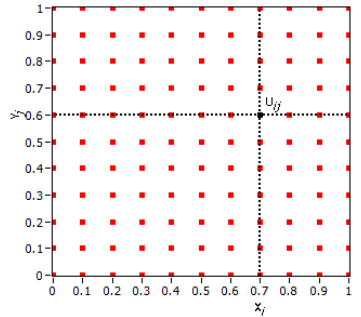
\includegraphics[width=\textwidth/2]{images/5-10-diskretizace.png}
        \caption*{Diskrerizace}
    \end{figure*}

    Počet uzlů na ose x označíme $n_x$, na ose y $n_y$.\\
    Pak dostaneme $h_x = \frac{1}{n_x+2},h_y = \frac{1}{n_y+2}$

    Diskretizací \eqref{eq:poisson} pak dostáváme
    \begin{equation}
        -\frac{u_{i+1,j} - 2u_{i,j} + u_{i-1,j}}{h_x^2} -\frac{u_{i,j+1} - 2u_{i,j} + u_{i,j-1}}{h_y^2} = f_{i,j}
    \end{equation} 
    Předpokládáme $n_x = n_y \implies h_x = h_y := h$ a dostaneme 

    \begin{equation*}
        \frac{1}{h^2} \begin{pmatrix}
            4 & -1 & 0 & 0 & -1 & 0 & 0 & 0 \\
            -1 & 4 & -1 & 0 & 0 & -1 & 0 & 0 \\
            0 & -1 & 4 & -1 & 0 & 0 & -1 & 0 \\
            0 & 0 & -1 & 4 & -1 & 0 & 0 & -1 \\
            -1 & 0 & 0 & -1 & 4 & -1 & 0 & 0 \\
            0 & -1 & 0 & 0 & -1 & 4 & -1 & 0 \\
            0 & 0 & -1 & 0 & 0 & -1 & 4 & -1 \\
            0 & 0 & 0 & -1 & 0 & 0 & -1 & 4 
            \end{pmatrix} = \dots
    \end{equation*}

    Ale pokud například $n_x = n_y = 1000 \implies n=10^6$ vrcholů.\\
    Při hustém uložení $n^2$ prvků $10^12$, pokud 8 bajtů na prvek $\implies$ 8TB dat.

    Vkládáme-li pouze nenulové prvky (tj. jen 5 diagonál kterých vzniká) $\approx 5*n$ prvků po 8B $\implies$ 40MB dat
\end{example}


\section{Reprezentace řídkých matic v počítači}
\subsection{Souřadnicový formát}
\begin{itemize}
    \item 1 pole reálných čísel délky $n_z$ (počet nenulových prvků v matici), 
    obsahující hodnoty nenulových prvků matice $\mathbf{A}$ v libovolném pořadí.
    \item 2 pole celých čísel obsahující řádkové, resp. sloupcové indexy nenulových prvků.
\end{itemize}

\begin{example}
    \begin{equation}\label{eq:sparse_example}
        \mathbf{A} = \begin{pmatrix}
            1 & 0 & 0 & 2 & 0 \\
            3 & 4 & 0 & 5 & 0 \\
            6 & 0 & 7 & 8 & 9 \\
            0 & 0 & 10 & 11 & 0 \\
            0 & 0 & 0 & 0 & 12 
            \end{pmatrix} 
    \end{equation}

Pak dostáváme následující 3 pole
\begin{align*}
    A\mathbf{A} &= (1,2,3,4,5,6,7,8,9,10,11,12)\\
    I\mathbf{A} &= (1,1,2,2,2,3,3,3,3,4,4,5)\\
    J\mathbf{A} &= (1,4,1,2,4,1,3,4,5,3,4,5)
\end{align*}

Lze vylepšit pokud ukládáme prvky systematicky (například po řádkách), pak $I\mathbf{A}$ obsahuje redundantní informaci.

\end{example}


\subsection{CSR formát (Compressed Sparse Rows)}

\begin{itemize}
    \item $A\mathbf{A}$ pole reálných čísel délky $n_z$ obsahující nenulové prvky matice $\mathbf{A}$ zapsané po řádcích.
    \item $J\mathbf{A}$ pole celých čísel délky $n_z$, obsahující sloupcové indexy prvků v $A\mathbf{A}$
    \item $I\mathbf{A}$ pole délky $n + 1$  (počet řádků $+1$), kde i-tý prvek udává index začátku i-tého řádku matice $\mathbf{A}$ v polích $A\mathbf{A}$ a $J\mathbf{A}$
\end{itemize}


\begin{example}
    Vezměme matici z \eqref{eq:sparse_example}, pak dostaneme
    \begin{align*}
        A\mathbf{A} &= (1,2,3,4,5,6,7,8,9,10,11,12)\\
        J\mathbf{A} &= (1,4,1,2,4,1,3,4,5,3,4,5)\\
        I\mathbf{A} &= (1,3,6,10,12,13)
    \end{align*}
    Poslední člen v $I\mathbf{A}$ (zde 13) je umělý ukazatel za konec $A\mathbf{A}$ a $J\mathbf{A}$

\end{example}
Výhody: \begin{itemize}
    \item Šetří paměť
    \item Cache hits
\end{itemize}

Nevýhody: \begin{itemize}
    \item Špatně se přidávají nenulové prvky
\end{itemize}

Existuje i alternativa, kdy matici ukládáme po sloupcích, tzv. CSC formát.


\subsection{MSR formát (Modified Sparse Rows)}

Často jsou diagonální prvky \matA nenulové a jsou potřeba častěji než ostatní prvky, proto ji uložíme zvlášť.




\begin{itemize}
    \item $A\mathbf{A}$ pole reálných čísel délky $n_z +1$ obsahující nenulové prvky matice $\mathbf{A}$ zapsané po řádcích.
    \item $J\mathbf{A}$ pole celých čísel délky $n_z +1$, obsahující sloupcové indexy prvků v $A\mathbf{A}$
    
\end{itemize}

\begin{example}
    Vezměme opět matici z \eqref{eq:sparse_example}, pak dostaneme
    
    \begin{align*}
        A\mathbf{A} &= (1,4,7,11,12,\star,2,3,5,6,8,9,10)\\
        J\mathbf{A} &= (7,8,10,13,14,\mathbf{14},4,1,4,1,4,5,3)
    \end{align*}

    V $A\mathbf{A}$ jsou tedy nejprve zapsané všechny diagonální prvky, jedno volné místo ($\star$) \\
    a ostatní nenulové prvky zapsané po řádcích

    V $J\mathbf{A}$ máme před $\mathbf{14}$ indexy začátků řádků v poli $A\mathbf{A}$, $\mathbf{14}$ je umělý ukazatel\\
    za konec pole $A\mathbf{A}$, za máme sloupcové indexy nediagonálních prvků
\end{example}



\subsection{Ellpack - Hpack}
Pro matice, které mají omezený počet nenulových prvků na 1 řádek, maximálně nějaké $N_d$, uvažujeme malé.


\begin{itemize}
    \item $COEF$ pole reálných čísel délky $n * N_d$ obsahuje na i-tém řádku (pokud máme 2D pole) hodnoty nenulových prvků
    i-tého řádku matice $\mathbf{A}$.
    \item $ICOEF$ obsahuje sloupcové indexy odpovídajících prvků v poli $COEF$
\end{itemize}


\begin{example}
    \begin{equation}\label{eq:example-diagonal}
        \mathbf{A} = \begin{pmatrix}
            1 & 0 & 2 & 0 & 0 \\
            3 & 4 & 0 & 5 & 0 \\
            0 & 6 & 7 & 0 & 8 \\
            0 & 0 & 9 & 10 & 0 \\
            0 & 0 & 0 & 11 & 12 
            \end{pmatrix}
    \end{equation}

    Vezměme $N_d = 3$, pak máme
    
    \begin{equation*}
        COEF = \begin{pmatrix}
            1 & 2 & \cdot \\
            3 & 4 & 5 \\
            6 & 7 & 8 \\
            9 & 10 & \cdot \\
            11 & 12 & \cdot 
            \end{pmatrix}
        , ICOEF = \begin{pmatrix}
            1 & 3 & \cdot \\
            1 & 2 & 4 \\
            2 & 3 & 5 \\
            3 & 4 & \cdot \\
            4 & 5 & \cdot 
            \end{pmatrix} 
    \end{equation*}    
\end{example}

\subsection{Diagonální uložení}
Jedná se tedy o matice v nichž se nenulové prvky nachází jen na několika málo diagonálách.

Nenulové diagonály matice \matA jsou uloženy v poli $DIAG$ velikosti $n*N_diag$.\\
Offsety každé diagonály jsou v poli $IOFF$, což je celočíselné pole délky $N_diag$\\
$DIAG[i,j]$ obsahuje $\mathbf{A}_{i,i+IOFF[j]}$

\begin{example}
    Příklad pro matici \eqref{eq:example-diagonal}


\begin{equation*}
    DIAG = \begin{pmatrix}
        1 & \star & 2 \\
        4 & 3 & 5 \\
        7 & 6 & 8 \\
        10 & 9 & \star \\
        12 & 11 & \star 
        \end{pmatrix}, IOFF = (0, -1, 2)
\end{equation*}

\end{example}





\end{document}